
%% bare_conf.tex
%% V1.3
%% 2007/01/11
%% by Michael Shell
%% See:
%% http://www.michaelshell.org/
%% for current contact information.
%%
%% This is a skeleton file demonstrating the use of IEEEtran.cls
%% (requires IEEEtran.cls version 1.7 or later) with an IEEE conference paper.
%%
%% Support sites:
%% http://www.michaelshell.org/tex/ieeetran/
%% http://www.ctan.org/tex-archive/macros/latex/contrib/IEEEtran/
%% and
%% http://www.ieee.org/

%%*************************************************************************
%% Legal Notice:
%% This code is offered as-is without any warranty either expressed or
%% implied; without even the implied warranty of MERCHANTABILITY or
%% FITNESS FOR A PARTICULAR PURPOSE! 
%% User assumes all risk.
%% In no event shall IEEE or any contributor to this code be liable for
%% any damages or losses, including, but not limited to, incidental,
%% consequential, or any other damages, resulting from the use or misuse
%% of any information contained here.
%%
%% All comments are the opinions of their respective authors and are not
%% necessarily endorsed by the IEEE.
%%
%% This work is distributed under the LaTeX Project Public License (LPPL)
%% ( http://www.latex-project.org/ ) version 1.3, and may be freely used,
%% distributed and modified. A copy of the LPPL, version 1.3, is included
%% in the base LaTeX documentation of all distributions of LaTeX released
%% 2003/12/01 or later.
%% Retain all contribution notices and credits.
%% ** Modified files should be clearly indicated as such, including **
%% ** renaming them and changing author support contact information. **
%%
%% File list of work: IEEEtran.cls, IEEEtran_HOWTO.pdf, bare_adv.tex,
%% bare_conf.tex, bare_jrnl.tex, bare_jrnl_compsoc.tex
%%*************************************************************************

% *** Authors should verify (and, if needed, correct) their LaTeX system ***
% *** with the testflow diagnostic prior to trusting their LaTeX platform ***
% *** with production work. IEEE's font choices can trigger bugs that do ***
% *** not appear when using other class files. ***
% The testflow support page is at:
% http://www.michaelshell.org/tex/testflow/



% Note that the a4paper option is mainly intended so that authors in
% countries using A4 can easily print to A4 and see how their papers will
% look in print - the typesetting of the document will not typically be
% affected with changes in paper size (but the bottom and side margins will).
% Use the testflow package mentioned above to verify correct handling of
% both paper sizes by the user's LaTeX system.
%
% Also note that the "draftcls" or "draftclsnofoot", not "draft", option
% should be used if it is desired that the figures are to be displayed in
% draft mode.
%
\documentclass[conference]{IEEEtran}
% Add the compsoc option for Computer Society conferences.
%
% If IEEEtran.cls has not been installed into the LaTeX system files,
% manually specify the path to it like:
% \documentclass[conference]{../sty/IEEEtran}

\usepackage{graphicx}
\usepackage{datetime}
\usepackage{cite}
\usepackage[hyphens]{url}
\usepackage[hidelinks]{hyperref}
\usepackage{csquotes}
\usepackage{array}
\usepackage {adjustbox}
\usepackage{tcolorbox}
\usepackage{graphicx}
\usepackage{multirow}
\usepackage{multicol}
\usepackage{pdflscape}
\usepackage{amsmath}
\usepackage{float}
\usepackage{afterpage}
\graphicspath{ {images/} }
\hypersetup{breaklinks=true}
\newcommand{\subparagraph}{}
\usepackage{titlesec}
\setcounter{secnumdepth}{4}

% Some very useful LaTeX packages include:
% (uncomment the ones you want to load)


% *** MISC UTILITY PACKAGES ***
%
%\usepackage{ifpdf}
% Heiko Oberdiek's ifpdf.sty is very useful if you need conditional
% compilation based on whether the output is pdf or dvi.
% usage:
% \ifpdf
% % pdf code
% \else
% % dvi code
% \fi
% The latest version of ifpdf.sty can be obtained from:
% http://www.ctan.org/tex-archive/macros/latex/contrib/oberdiek/
% Also, note that IEEEtran.cls V1.7 and later provides a builtin
% \ifCLASSINFOpdf conditional that works the same way.
% When switching from latex to pdflatex and vice-versa, the compiler may
% have to be run twice to clear warning/error messages.






% *** CITATION PACKAGES ***
%
%\usepackage{cite}
% cite.sty was written by Donald Arseneau
% V1.6 and later of IEEEtran pre-defines the format of the cite.sty package
% \cite{} output to follow that of IEEE. Loading the cite package will
% result in citation numbers being automatically sorted and properly
% "compressed/ranged". e.g., [1], [9], [2], [7], [5], [6] without using
% cite.sty will become [1], [2], [5]--[7], [9] using cite.sty. cite.sty's
% \cite will automatically add leading space, if needed. Use cite.sty's
% noadjust option (cite.sty V3.8 and later) if you want to turn this off.
% cite.sty is already installed on most LaTeX systems. Be sure and use
% version 4.0 (2003-05-27) and later if using hyperref.sty. cite.sty does
% not currently provide for hyperlinked citations.
% The latest version can be obtained at:
% http://www.ctan.org/tex-archive/macros/latex/contrib/cite/
% The documentation is contained in the cite.sty file itself.






% *** GRAPHICS RELATED PACKAGES ***
%
\ifCLASSINFOpdf
% \usepackage[pdftex]{graphicx}
% declare the path(s) where your graphic files are
% \graphicspath{{../pdf/}{../jpeg/}}
% and their extensions so you won't have to specify these with
% every instance of \includegraphics
% \DeclareGraphicsExtensions{.pdf,.jpeg,.png}
\else
% or other class option (dvipsone, dvipdf, if not using dvips). graphicx
% will default to the driver specified in the system graphics.cfg if no
% driver is specified.
% \usepackage[dvips]{graphicx}
% declare the path(s) where your graphic files are
% \graphicspath{{../eps/}}
% and their extensions so you won't have to specify these with
% every instance of \includegraphics
% \DeclareGraphicsExtensions{.eps}
\fi
% graphicx was written by David Carlisle and Sebastian Rahtz. It is
% required if you want graphics, photos, etc. graphicx.sty is already
% installed on most LaTeX systems. The latest version and documentation can
% be obtained at: 
% http://www.ctan.org/tex-archive/macros/latex/required/graphics/
% Another good source of documentation is "Using Imported Graphics in
% LaTeX2e" by Keith Reckdahl which can be found as epslatex.ps or
% epslatex.pdf at: http://www.ctan.org/tex-archive/info/
%
% latex, and pdflatex in dvi mode, support graphics in encapsulated
% postscript (.eps) format. pdflatex in pdf mode supports graphics
% in .pdf, .jpeg, .png and .mps (metapost) formats. Users should ensure
% that all non-photo figures use a vector format (.eps, .pdf, .mps) and
% not a bitmapped formats (.jpeg, .png). IEEE frowns on bitmapped formats
% which can result in "jaggedy"/blurry rendering of lines and letters as
% well as large increases in file sizes.
%
% You can find documentation about the pdfTeX application at:
% http://www.tug.org/applications/pdftex





% *** MATH PACKAGES ***
%
%\usepackage[cmex10]{amsmath}
% A popular package from the American Mathematical Society that provides
% many useful and powerful commands for dealing with mathematics. If using
% it, be sure to load this package with the cmex10 option to ensure that
% only type 1 fonts will utilized at all point sizes. Without this option,
% it is possible that some math symbols, particularly those within
% footnotes, will be rendered in bitmap form which will result in a
% document that can not be IEEE Xplore compliant!
%
% Also, note that the amsmath package sets \interdisplaylinepenalty to 10000
% thus preventing page breaks from occurring within multiline equations. Use:
%\interdisplaylinepenalty=2500
% after loading amsmath to restore such page breaks as IEEEtran.cls normally
% does. amsmath.sty is already installed on most LaTeX systems. The latest
% version and documentation can be obtained at:
% http://www.ctan.org/tex-archive/macros/latex/required/amslatex/math/





% *** SPECIALIZED LIST PACKAGES ***
%
%\usepackage{algorithmic}
% algorithmic.sty was written by Peter Williams and Rogerio Brito.
% This package provides an algorithmic environment fo describing algorithms.
% You can use the algorithmic environment in-text or within a figure
% environment to provide for a floating algorithm. Do NOT use the algorithm
% floating environment provided by algorithm.sty (by the same authors) or
% algorithm2e.sty (by Christophe Fiorio) as IEEE does not use dedicated
% algorithm float types and packages that provide these will not provide
% correct IEEE style captions. The latest version and documentation of
% algorithmic.sty can be obtained at:
% http://www.ctan.org/tex-archive/macros/latex/contrib/algorithms/
% There is also a support site at:
% http://algorithms.berlios.de/index.html
% Also of interest may be the (relatively newer and more customizable)
% algorithmicx.sty package by Szasz Janos:
% http://www.ctan.org/tex-archive/macros/latex/contrib/algorithmicx/




% *** ALIGNMENT PACKAGES ***
%
%\usepackage{array}
% Frank Mittelbach's and David Carlisle's array.sty patches and improves
% the standard LaTeX2e array and tabular environments to provide better
% appearance and additional user controls. As the default LaTeX2e table
% generation code is lacking to the point of almost being broken with
% respect to the quality of the end results, all users are strongly
% advised to use an enhanced (at the very least that provided by array.sty)
% set of table tools. array.sty is already installed on most systems. The
% latest version and documentation can be obtained at:
% http://www.ctan.org/tex-archive/macros/latex/required/tools/


%\usepackage{mdwmath}
%\usepackage{mdwtab}
% Also highly recommended is Mark Wooding's extremely powerful MDW tools,
% especially mdwmath.sty and mdwtab.sty which are used to format equations
% and tables, respectively. The MDWtools set is already installed on most
% LaTeX systems. The lastest version and documentation is available at:
% http://www.ctan.org/tex-archive/macros/latex/contrib/mdwtools/


% IEEEtran contains the IEEEeqnarray family of commands that can be used to
% generate multiline equations as well as matrices, tables, etc., of high
% quality.


%\usepackage{eqparbox}
% Also of notable interest is Scott Pakin's eqparbox package for creating
% (automatically sized) equal width boxes - aka "natural width parboxes".
% Available at:
% http://www.ctan.org/tex-archive/macros/latex/contrib/eqparbox/





% *** SUBFIGURE PACKAGES ***
%\usepackage[tight,footnotesize]{subfigure}
% subfigure.sty was written by Steven Douglas Cochran. This package makes it
% easy to put subfigures in your figures. e.g., "Figure 1a and 1b". For IEEE
% work, it is a good idea to load it with the tight package option to reduce
% the amount of white space around the subfigures. subfigure.sty is already
% installed on most LaTeX systems. The latest version and documentation can
% be obtained at:
% http://www.ctan.org/tex-archive/obsolete/macros/latex/contrib/subfigure/
% subfigure.sty has been superceeded by subfig.sty.



%\usepackage[caption=false]{caption}
%\usepackage[font=footnotesize]{subfig}
% subfig.sty, also written by Steven Douglas Cochran, is the modern
% replacement for subfigure.sty. However, subfig.sty requires and
% automatically loads Axel Sommerfeldt's caption.sty which will override
% IEEEtran.cls handling of captions and this will result in nonIEEE style
% figure/table captions. To prevent this problem, be sure and preload
% caption.sty with its "caption=false" package option. This is will preserve
% IEEEtran.cls handing of captions. Version 1.3 (2005/06/28) and later 
% (recommended due to many improvements over 1.2) of subfig.sty supports
% the caption=false option directly:
%\usepackage[caption=false,font=footnotesize]{subfig}
%
% The latest version and documentation can be obtained at:
% http://www.ctan.org/tex-archive/macros/latex/contrib/subfig/
% The latest version and documentation of caption.sty can be obtained at:
% http://www.ctan.org/tex-archive/macros/latex/contrib/caption/




% *** FLOAT PACKAGES ***
%
%\usepackage{fixltx2e}
% fixltx2e, the successor to the earlier fix2col.sty, was written by
% Frank Mittelbach and David Carlisle. This package corrects a few problems
% in the LaTeX2e kernel, the most notable of which is that in current
% LaTeX2e releases, the ordering of single and double column floats is not
% guaranteed to be preserved. Thus, an unpatched LaTeX2e can allow a
% single column figure to be placed prior to an earlier double column
% figure. The latest version and documentation can be found at:
% http://www.ctan.org/tex-archive/macros/latex/base/



%\usepackage{stfloats}
% stfloats.sty was written by Sigitas Tolusis. This package gives LaTeX2e
% the ability to do double column floats at the bottom of the page as well
% as the top. (e.g., "\begin{figure*}[!b]" is not normally possible in
% LaTeX2e). It also provides a command:
%\fnbelowfloat
% to enable the placement of footnotes below bottom floats (the standard
% LaTeX2e kernel puts them above bottom floats). This is an invasive package
% which rewrites many portions of the LaTeX2e float routines. It may not work
% with other packages that modify the LaTeX2e float routines. The latest
% version and documentation can be obtained at:
% http://www.ctan.org/tex-archive/macros/latex/contrib/sttools/
% Documentation is contained in the stfloats.sty comments as well as in the
% presfull.pdf file. Do not use the stfloats baselinefloat ability as IEEE
% does not allow \baselineskip to stretch. Authors submitting work to the
% IEEE should note that IEEE rarely uses double column equations and
% that authors should try to avoid such use. Do not be tempted to use the
% cuted.sty or midfloat.sty packages (also by Sigitas Tolusis) as IEEE does
% not format its papers in such ways.





% *** PDF, URL AND HYPERLINK PACKAGES ***
%
%\usepackage{url}
% url.sty was written by Donald Arseneau. It provides better support for
% handling and breaking URLs. url.sty is already installed on most LaTeX
% systems. The latest version can be obtained at:
% http://www.ctan.org/tex-archive/macros/latex/contrib/misc/
% Read the url.sty source comments for usage information. Basically,
% \url{my_url_here}.





% *** Do not adjust lengths that control margins, column widths, etc. ***
% *** Do not use packages that alter fonts (such as pslatex). ***
% There should be no need to do such things with IEEEtran.cls V1.6 and later.
% (Unless specifically asked to do so by the journal or conference you plan
% to submit to, of course. )


% correct bad hyphenation here
\hyphenation{op-tical net-works semi-conduc-tor}


\begin{document}
%
% paper title
% can use linebreaks \\ within to get better formatting as desired
%\title{On the Impact of Security Questions on Answers}
%\title{``secret question meter": A visual interface design nudges users towards stronger answers in security questions}
\title{%
Title : \textit{subtitle} }
% author names and affiliations
% use a multiple column layout for up to three different
% affiliations

%\author{\IEEEauthorblockN{Awanthika Rasanjalee Senarath\IEEEauthorrefmark{1},
%and Nalin A.G. Arachchilage \IEEEauthorrefmark{2} }
%\IEEEauthorblockA{Australian Centre for Cyber Security\\
%University of New South Wales Canberra\\
%Australian Defence Force Academy\\
%Email: \IEEEauthorrefmark{1}a.senarath@student.unsw.edu.au,
%\IEEEauthorrefmark{2}nalin.asanka@adfa.edu.au
%}}




% conference papers do not typically use \thanks and this command
% is locked out in conference mode. If really needed, such as for
% the acknowledgment of grants, issue a \IEEEoverridecommandlockouts
% after \documentclass

% for over three affiliations, or if they all won't fit within the width
% of the page, use this alternative format:
% 
%\author{\IEEEauthorblockN{Michael Shell\IEEEauthorrefmark{1},
%Homer Simpson\IEEEauthorrefmark{2},
%James Kirk\IEEEauthorrefmark{3}, 
%Montgomery Scott\IEEEauthorrefmark{3} and
%Eldon Tyrell\IEEEauthorrefmark{4}}
%\IEEEauthorblockA{\IEEEauthorrefmark{1}School of Electrical and Computer Engineering\\
%Georgia Institute of Technology,
%Atlanta, Georgia 30332--0250\\ Email: see http://www.michaelshell.org/contact.html}
%\IEEEauthorblockA{\IEEEauthorrefmark{2}Twentieth Century Fox, Springfield, USA\\
%Email: homer@thesimpsons.com}
%\IEEEauthorblockA{\IEEEauthorrefmark{3}Starfleet Academy, San Francisco, California 96678-2391\\
%Telephone: (800) 555--1212, Fax: (888) 555--1212}
%\IEEEauthorblockA{\IEEEauthorrefmark{4}Tyrell Inc., 123 Replicant Street, Los Angeles, California 90210--4321}}




% use for special paper notices
%\IEEEspecialpapernotice{(Invited Paper)}




% make the title area
\maketitle

\begin{abstract}
%\boldmath


\end{abstract}
% IEEEtran.cls defaults to using nonbold math in the Abstract.
% This preserves the distinction between vectors and scalars. However,
% if the conference you are submitting to favors bold math in the abstract,
% then you can use LaTeX's standard command \boldmath at the very start
% of the abstract to achieve this. Many IEEE journals/conferences frown on
% math in the abstract anyway.

% no keywords

% For peer review papers, you can put extra information on the cover
% page as needed:
% \ifCLASSOPTIONpeerreview
% \begin{center} \bfseries EDICS Category: 3-BBND \end{center}
% \fi
%
% For peerreview papers, this IEEEtran command inserts a page break and
% creates the second title. It will be ignored for other modes.
\IEEEpeerreviewmaketitle

\section{Introduction}

Disclosure of personal details into software systems (mobile apps, online web apps) always comes with an associated privacy risk. For example, every time a user taps his/her credit card into the payment system in the supermarket, s/he discloses information about his/her purchase to the system. The system can very easily process this data and determine the user's preferred brands, his/her weekly expenditure on groceries and predict how to target him/her with advertising. Therefore, when users disclose more data into software applications, the ways through which their privacy could be compromised increase. 

Software systems using collected data for reasons unforeseen by users and sharing data with third parties unknown to the user could result in privacy vulnerabilities \cite {malhotra2004internet}. Because of this, users are known to be reluctant to disclose data when they believe the associated privacy risk of disclosing data to the system is high \cite {kobsa2007privacy}. Therefore, disclosure decisions of users are closely related to privacy, as users disclose data when their perceived privacy risk is low  \cite {li2010understanding}. That is, users are most likely to disclose their data to a software system if they feel that the ways through which the system could compromise their privacy (data sharing, data selling) is minimum. Hence, understanding data disclosure decisions made by users in a given circumstance could help understanding perceived privacy risk by users. 

Privacy conscious users face many problems when they make decisions to disclose their information into software systems \cite {li2010understanding}. There exist many research that attempt to identify what affect the disclosure decisions made by users in order to increase information disclosure by users, to understand user perception and satisfaction in data disclosure \cite {knijnenburg2013making}. These approaches to observe decisions made by users when they disclose data into systems, focus either on the properties of the application that requests data \cite {li2010understanding, wang2016context, malheiros2013fairly} or the personality of the user who discloses data \cite {nissenbaum2009privacy}. These research have sometimes identified properties of the data items being disclosed to have an effect on data disclosure decisions made by users. For example, properties of data users disclose to a system, such as : how sensitive is this data? and how relevant is this data to the application? are known to have an effect on the disclosure decisions of users \cite {malheiros2013fairly}. 

Knowledge of the effect of the properties of data being collected on the data disclosure decisions of users could help building up a metric for privacy risk of data items \cite {maximilien2009privacy}. Such a privacy metric that communicates the associated privacy risk of data items could help software developers to decide which data to collect, which data to store and how to store and process user data in a system when they design software systems. Similarly, with a privacy measurement metric on data items researchers and law makers can make better regulations and privacy practices that would relate privacy with the user data.

In this research we attempt to extract how users perceive different aspects of data that leads to their decisions in disclosing their data into software systems. Using a survey with 151 respondents we observe how users perceive the sensitivity of the data items to the user, relatedness of the data items to the purpose of an application and the visibility a particular data item gets in an application when they decide to disclose their data into software systems. With this knowledge we attempt to build a relationship relating how sensitivity, visibility and relatedness of data items relate to perceived user privacy risk. Furthermore, through a qualitative analysis we attempt to identify other factors, if any, that could affect users data disclosure decisions.

This paper has the following contribution.

\begin{itemize}
\item Constructing a metric to measure associated privacy risk of data items in a given context. A metric to measure privacy of data that takes into account the context in which it is disclosed (by considering the relatedness of the data item to the application context) would help software developers to make decisions about collecting, storing and using different data items in software systems. 
\end{itemize}

The paper is structured as follows. We first discuss previous work that has identified the parameters (sensitivity, visibility and relatedness) in measuring privacy in the background section. Then we describe our user study followed by the results. Next, we discuss the implications of our findings followed by the conclusion and future work.

\section {Related work}

Most research that focus on user disclosure decisions have the motivation to increase user data disclosure. These research focus on what makes users disclose more data rather than understanding how users disclose data. For example, Besmer et al. said that users are more likely to decide to disclose data when they are shown the decisions made by other users \cite {besmer2010impact} Similarly, Dennett has said that users feel comfortable sharing their data when they are shown the decisions made by their friends. \cite {dennett2000little}. Furthermore, Acquisti et al. found that changing the order of intrusiveness of the data being requested also makes users disclose more data when interacting with software systems \cite {acquisti2012impact}. Similarly, testing the effect of the justification provided by the system when requesting data Knijnenburg and Kobsa \cite {knijnenburg2013helping} revealed that when users are told \textit{this data is useful for you} users are more likely to disclose data with the application. Interestingly, all these research focus on system behaviors (way of requesting data, justification for data collection) and user's personal preferences ( users' experience with a system, users' expectation from a system) and their effects on user data disclosure decisions.

Particularly focusing on the intrinsic properties of the data being shared, Bansal et al. have shown that users' intention to disclose health information is affected by the sensitivity of the data\cite {bansal2010impact}. Malhotra et al have shown that consumer willingness to share personal data in commercial platforms is affected by the sensitivity of the data \cite {malhotra2004internet}. Similarly, Malheiros et al. \cite {malheiros2013fairly} have shown that sensitivity of data items such as date of birth and occupation had a significant affect on disclosure. They have also identified an effect of data relevance for a given application context on disclosure decisions made by users. However, no effort has been made so far to communicate this effect in a way that could help software developers and privacy researchers to relate data with user disclosure decisions.

Particularly focusing on privacy risk, Maximilien et al. \cite {maximilien2009privacy} have shown that a metric for privacy in a given context can be obtained by multiplying the measurement for sensitivity of a data item with the measurement for visibility the data item gets in an application. They define their metric for privacy as \enquote{a measurement that determines their [the user's ]willingness to disclose information associated with this item} \cite {maximilien2009privacy}. Using the same metric, Minkus and Memon \cite{minkus2014scale} have attempted to measure user privacy from users' Facebook privacy settings. They have shown that the metric could be used to measure the privateness of a user from the choices s/he makes when setting up the privacy settings in Facebook. However, this is a contextual measurements. The context in which data is being disclosed \cite {nissenbaum2009privacy, john2010strangers} is known to have an effect on user disclosure decisions \cite {knijnenburg2013making}. For example, it is said that users have an undermining effect on rewards for data disclosure when the requested data appears irrelevant for a system \cite {li2010understanding}, whereas they accepted the rewards if the data is relevant for the system. Therefore, a holistic measurement for privacy also needs to consider data relevance when measuring user privacy from the data disclosure decisions. 

We focus on investigating the effect of data sensitivity, the relevance of the data for an application and the visibility the data gets in the application on user disclosure decisions. With this we focus on obtaining a privacy risk metric in order to communicate the effect of data sensitivity, visibility and the relatedness of data for a particular application on user disclosure decisions to software developers and privacy researchers. This metric would help software developers to understand and incorporate perceived privacy risk of users into the software system designs and assist the development of privacy preserving software systems. For example, developers could identify which data users are most concerned about and which data users would feel most uncomfortable sharing. This knowledge could help them implement better security for data in system designs and communicate it to the user in order to make users comfortable sharing data with the system.


\section {Methodology}

In this section we first introduce the parameters we are measuring in this research. Then we will build the relationship we propose based on existing knowledge. Then we will discuss the user study we conducted to evaluate the relationship propose, our findings and the correlations.

\subsection {Notations}

The goal of our research was to calculate the relationship between sensitivity (S), relatedness (R) and visibility (V) of data on the feeling of discomfort when users make the disclosure decisions. For this we define sensitivity, visibility and relatedness of data to be parameters that depend only on a particular data item \textit{$D_i$} and the application ontext in which it is being used \textit{$C_j$}.

\subsubsection{Data Sensitivity} We define the sensitivity of a particular data item to be a parameter that is dependent on the data item \textit{$D_i$} itself. That is inherently for a user their credit card number is ore sensitive than their age. We define sesitivity of a data item to be the perceived impact of loss of that particular data item. We define sensitivity in three categorical values. That is, 

\begin{center}
\begin{table}[htbp]
\caption{Participant Gender Distribution}
\begin{center}
\begin{adjustbox}{width=0.5\textwidth} 
\begin{tabular}{|p{0.2\linewidth}|p{0.7\linewidth}|p{0.1\linewidth}|} 
\hline
Category & Description & Sensitivity Value \\
\hline
Category I - Highest sesntivity & Data that could be used to identify a unique characteristic of a person. For example, a person's race, religion or HIV status. & 3 \\
\hline
Category II - Moderate sensitivity & Personally Identifiable information about the person. For example, a person's name, address, mobile number & 2 \\
\hline
Catwgory III - Low sensitivity & Any other detail about a person that may have an impact of loss, however, would not affect the person. For example, a person's high school & 1 \\
\hline
\end{tabular}
\end{adjustbox}
\end{center}
\end{table}
\end{center} 

Therefore according to our definition the sensitivity of a data element \textit {$D_i$} takes categorical values S $\in$ \{1,2,3\}.

\subsubsection {Data visibility} We define the visibility of a data element to be an inherent property gained by a particular data element \textit{$D_i$} in a particular application context \textit{$C_j$} due to the design of the application. That is how visible the data item would be by default once the user disclose the data item to the application. If the application by default allows the data to be seen only by the user, we define that data item has the lowest visibility.  

\begin{center}
\begin{table}[htbp]
\caption{Participant Gender Distribution}
\begin{center}
\begin{adjustbox}{width=0.5\textwidth} 
\begin{tabular}{|p{0.2\linewidth}|p{0.7\linewidth}|p{0.1\linewidth}|} 
\hline
Category & Description & Visibility Value \\
\hline
Category I - Highest visibility & Data would be seen by any one by default. Data is visible in the application by default. For example the name of a user in Facebook & 3 \\
\hline
Category II - Moderate visibility & Data would be seen by a controlled set of users by default. For example,   & 2 \\
\hline
Catwgory III - Low visibility & Data would be seen by any one by default. Data is visible in the application by default. For example, your pin number in the banking app will not be visible to anyone & 1 \\
\hline
\end{tabular}
\end{adjustbox}
\end{center}
\end{table}
\end{center} 

Therefore according to our definition the visibility of a data element \textit {$D_i$} in an application context textit {$C_j$} takes categorical values V $\in$ \{1,2,3\}.

\subsubsection {Data Relatedness} We define the relateness of a data element \textit {$D_i$} to be a property that is defined by the application context \textit {$C_j$}. That is based on the requirements of the application, the data could be highly related to the application (For example, your bank account number for your banking application) or no related at all. This is determined by the primary functionality of the application defined by the application requirements.

\begin{center}
\begin{table}[htbp]
\caption{Participant Gender Distribution}
\begin{center}
\begin{adjustbox}{width=0.5\textwidth} 
\begin{tabular}{|p{0.2\linewidth}|p{0.7\linewidth}|p{0.1\linewidth}|} 
\hline
Category & Description & Relatedness Value \\
\hline
Category I - Highest relatedness & Data the application cannot do without. These data ara absolutely necessary for the primary functionality of the application & 3 \\
\hline
Category II - Moderate relatedness & Data could add additional functionality to the application. For example, data that could deliver benefits through data analysis techniques & 2 \\
\hline
Catwgory III - Low relatedness & Data the application can do without. & 1 \\
\hline
\end{tabular}
\end{adjustbox}
\end{center}
\end{table}
\end{center} 
Therefore according to our definition the relatedness of a data element \textit {$D_i$} in an application context \textit {$C_j$} also takes categorical values R $\in$ \{1,2,3\}.

\subsubsection {Calculated privacy risk of a data element \textit {$D_i$} in an application context \textit {$C_j$} } We then define the calculated privacy risk \textit{$P_c$} of a data element \textit {$D_i$} in an application context \textit {$C_j$} as follows. Building up on the relationship proposed by Maximilien et al. \cite {maximilien2009privacy} we define that the privacy risk \textit{$P_c$} of a data element \textit {$D_i$} in an application context \textit {$C_j$}  monotonicall increases with the sensitivity of a data item \textit{$S_i$} and the visibility of a data item in a given context \textit{$V_{(i,j)}$}. This has been previously used by Minkus and Memon \cite{minkus2014scale} in determining the privacy level of Facebook privacy settings for a particular user. Based on this, we propose that the privacy risk \textit{$P_c$} of a data element \textit {$D_i$} in an application context \textit {$C_j$} is in a monotonically decremental relationship with the relatedness of the data element \textit {$D_i$} to the application context \textit {$C_j$}. This is based on the logic that users perceive low privacy risk when discosing data items that are relevant to the applicationo as opposed to data elements that do not appear relevant. Therefore, we propose that an approximation for the privacy risk \textit{$P_c$} of a data element \textit {$D_i$} in an application context \textit {$C_j$} can be obtained by,

\[
\text {Privacy Risk $P_(i,j)$} =\frac{S_{i}^a \times V_{(i,j)}^b}{R_{(i,j)}^ c}
\]

where a,b and c values could take any real number. However, as we are aiming for an approximation we limit a,b,c to whole numbers.

According to this calculation Privacy Risk $P_(i,j)$  of a data element \textit {$D_i$} in an application context \textit {$C_j$} $\in$ \{x$\mid$ x $in$ ${\rm I\!R}$ where, 0 $\leq$ x\}. This relationship could be used to measure the privacy risk of data in a given application context so that developers and system designers could get an idea as to how appropriate privacy measures should be implemented for data items in an application design. However, this is a logically proposed relationship. Even though the initial relationship proposed by Maximilien et al has been used in many research that attempts to measure privacy in different contexts, it has not yet been verified through empriccal evidence. Therefore, next we conduct a user study to observe how closely this relationship would approximate the actual perceived user privacy.


\subsection {Research Study}

Our goal in this research is to observe how the close the relationship we propossed using data sensitivity, visibility and relatedness approximate the actual perceveid privacy risk by users. Going along with Maximilien et al. \cite {maximilien2009privacy} we define perceived privacy risk to be \enquote{a measurement that determines the user's feeling of discomfort in disclosing information associated with a data item}. Therefore, we define Privacy Risk $P_(i,j)$ such that,

\[
\text{ $P_(i,j)$} = \text{user's feeling of discomfort in disclosing an data \\
 item \textit {$D_i$} in an application context \textit {$C_j$}}
\]

In order to obtain the discomfort of data disclosure of users we defined three application contexts and ten data elements. The application contexts we defined were,

\begin{itemize}
\item Health Care application - with data being visible to the user and xx
\item Social Networking application - with no control over data visibility (Cannot control who can view the data once disclosed)
\item Banking application - with the data being visible only to the user (and the bank)
\end{itemize}

We communicated three different visibility levels in the three application contexts. Then, we defined the data items including demographic data and sensitive data following the Data Protection Regulations. The data items we provided are name, age, address, mobile number, email address, occupation, blood type, credit card number, medicine taken, and birthday. We asked the participants how they would feel if they are to disclose these 10 data items in the four application contexts. We define a five point Likert scale to express their \textit{feeling of disclosure} $F_d$, with values, very uncomfortable, somewhat uncomfortable, neutral, somewhat comfortable and very comfortable. We alternatively used reverse ordered likert scales to ensure the validity of the answers. We consider $F_d$ to be a function of the sensitivity of the data item i ($S_i$), visibility of the data item in the application j ($V_j$) and the relatedness of the data item to the context of the software system j ($R_j$). Our goal is to determine how close the relationship we proposed approximate $F_d$.

Following these four questions we also included an open ended question in the questionnaire to further observe the reasons for the difference in the feeling of discomfort ($F_d$) users expressed. With this we aimed to obtain further insights as to why users demonstrate different discomfort levels when they disclose different data items into different application contexts. 

At the end of the survey, we included questions to extract the demographics of the participants. However, we included an option \textit{prefer not to say} in all these questions, so that users could avoid disclosing their age, gender and educational background.

Tables 1-3 provides the basic profile of the participants;

\begin{center}
\begin{table}[htbp]
\caption{Participant Gender Distribution}
\begin{center}
\begin{tabular}{|l|l|} 
\hline
Gender & No. of Participants \\
\hline
Male & 87 \\
\hline
Female & 64 \\
\hline
\end{tabular}
\end{center}
\end{table}
\end{center} 

\begin{center}
\begin{table}[htbp]
\caption{Participant Education Distribution}
\begin{center}

\begin{tabular}{|l|l|} 
\hline
Education & No. of Participants \\
\hline
Completed School Education & 5 \\
\hline
Professional Diploma & 9 \\
\hline
Bachelor's Degree & 87 \\
\hline
Masters/PhD & 50 \\
\hline
\end{tabular}
\end{center}
\end{table}
\end{center} 

\begin{center}
\begin{table}[htbp]
\caption{Participant Age Distribution}
\begin{center}
\begin{tabular}{|l|l|} 
\hline
Age & No. of Participants \\
\hline
18-24  & 31 \\
\hline
25-32 & 101 \\
\hline
33-40& 13 \\
\hline
41 or above & 6\\
\hline
\end{tabular}
\end{center}
\end{table}
\end{center} 

The survey design was evaluated with two participants (graduate students in the university not connected to the research). We fine tuned the wording of the questionnaire with the feedback of these two participants. Then the survey was distributed using social media platforms (Facebook, LinkedIn and Twitter) and personal connections of the authors. Before proceeding to the survey, participants were given a brief introduction about the survey and the duration of the survey (under 10 minutes, calculated using the participants who evaluated the questionnaire). We also provided the participants with the contact details of the researchers. The research methodology (survey design, participant recruitment and results collection) was approved by the university ethic committee responsible for ethical conduction of studies that involve human subjects. Before proceeding with the survey participants were given an introduction to the survey page with details about the survey and the type of data we collect. We also informed they that they could exit the survey at any time without submitting their answers. Participants were asked to proceed with the survey if they give consent to collect and store the details they submit with the survey.

We measured the participant adequacy while collecting data and stopped data collection once we reached sample adequacy at KMO = 0.8. We then analyzed the data to obtain results.

\subsection {Data Analysis}

We assigned values from 1 to 5 for the answers we received on the Likert scale as given in Table 04.

\begin{center}
\begin{table}[htbp]
\caption{Assigning values to Likert Scale preferences}
\begin{center}
\begin{tabular}{|l|l|} 
\hline
Likert Scale Preference & Value Assigned \\
\hline
Very Comfortable & 1\\
\hline
Somewhat Comfortable& 2 \\
\hline
Neutral & 3  \\
\hline
Somewhat Uncomfortable & 4 \\
\hline
Very Uncomfortable & 5 \\
\hline
\end{tabular}
\end{center}
\end{table}
\end{center}

Through this we obtained $F_d$ $\in$ \{1,2,3,4,5\}. Then we averaged $F_d$ across all 151 participants to obtain the mean perceived privacy risk of users for the 30 scenarios (ten data items in three application contexts).

Next, in order to see how our calculated privacy risk $P_(i,j)$ approximate the perceived privacy risk $F_d$, we need to obtain the values for $P_(i,j)$ for the ten data items in the three different application contexts. As our goal is to introduce a metric for software developers to evaluate the perceived privacy risk of users, we calculated $P_(i,j)$ through a focus group with 4 participants with a software development experience. We believe this approach would closely represent the context in which software developers would discuss and evaluate the sensitivity, visibility and the relatedness of the data elements they use in software systems, at design stage. 

We asked the participants to first take the data items as individual elements and vategorize them according to the sensitivity of the data item. We provided them with the three categories we used in table 01. Next, for all three application scenarios, we asked them to categorize the ten data items according to their relatedness to the application context. For this we provided them with table III. As sensitivity was pre-determined and communicated to users in the user study we did not evaluate it here. In the results section we present the different calculated privacy risk ($P_(i,j)$) values we obtained and the corresponding perceived privacy risk ($F_d$) values we compaired.

Finally used qualitative methods to analyze the answers to the open ended question. We first developed a coding scheme by summarizing the meaning of the answers  \cite {wong2017eliciting}. This was done in NVivo \cite {saldana2015coding}. We reached code saturation at 49 participants. Then using the coding scheme two independent coders coded the data. At this stage coders were encouraged to insert any new code they considered important in interpreting the data. However, no new codes were generated at the coding stage. Since the answers were not more than two sentences long the coding process was simple and straight forward. We did not require iterative merging of codes and we present the primary codes obtained when we present the qualitative results.

\section {Results}

We tested the validity of our results with Cronbach's alpha (0.91) (a Cronbach's alpha $>$ 0.7 is considered acceptable \cite {nunnally1967psychometric}) and the participant adequacy for correlations with KMO (KMO =  0.8269) (A KMO value $0.8$ is considered good in calculating correlations among parameters \cite {kim1978factor}). 

The following table shows the results when we tested different models for calculated privacy risk $P_(i,j)$ against the perceived privacy risk $F_d$. The model fitting was done in Matlab curve fitting app.

\begin{center}
\begin{table}[htbp]
\caption{Participant Gender Distribution}
\begin{center}
\begin{adjustbox}{width=0.5\textwidth} 
\begin{tabular}{|p{0.6\linewidth}|p{0.4\linewidth}|} 
\hline
Model & Goodness of Fit \\
\hline
scenario 1 : $\frac{S_{i}^1 \times V_{(i,j)}^1}{R_{(i,j)}^1}$ & SSE : 67.8  $R^2$ = 0.6 RMSE = 1.5 \\
\hline
scenario 2 : $\frac{S_{i}^2 \times V_{(i,j)}^2}{R_{(i,j)}^ 2}$ & SSE : 14.4  $R^2$  = 0.35 \\
\hline
scenario 3 : $\frac{S_{i}^3 \times V_{(i,j)}^3}{R_{(i,j)}^3}$ & SSE :  11.68  $R^2$ = 0.575  \\
\hline
\end{tabular}
\end{adjustbox}
\end{center}
\end{table}
\end{center} 

With these values, we can see that the relationship $\frac{S_{i}^3 \times V_{(i,j)}^3}{R_{(i,j)}^3}$ best represents the perceived privacy risk of users in a given application context. However, we also observed the outliers to the model to be somewhat high. This is because the mean values we obtained for $F_d$ had high standard deviations. That is , for the same S,V and R combination for a particular data point received an $F_d$ value of 1 from some users and 5 from some. Prevoius research has shown that the personality of a person has a significant contribution to th eperceived privacy risk of that person. It has been said that users could be profiled as privacy fundamentalists, privacy pragmatists and privacy unconerned according to their personalities. We believe the different $F_d$ values we obtained to be a result of this. In our research our focus was to model the perceived privayc risk eliminating the personality traits of a person. Therefore, by design we did not capture the privacy profile of our participants. However, when we establish a model to communicate the perceived privacy risk of users, for th emodel to be applicable for all users, we believe tha tidealy it should be based on the perceived privacy risk of privacy fundamentalists. In that case, the perceived privacy risk would be highest. If a system is designed to facilitate the privacy risks of privacy fundamentalists, it would by default facilitate the privacy requirements of all users. Therefore, as future work, we aim to run our study with privacy profiling of participants in order to observe how our model captures the privacy requirements of users with different privacy personalities. 









Following charts (image 1-4) shows the averages of the disclosure feeling of the 151 participants on the 10 data items across the three scenarios.

\begin{figure}[h]
\begin{center}
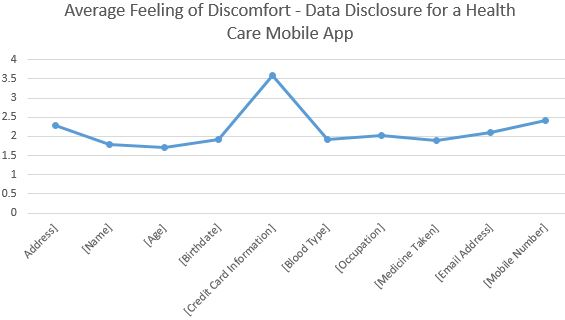
\includegraphics[width=0.5\textwidth]{Average_Health}
\caption{Feeling of Discomfort in Disclosure - Health  application}
\end{center}
\end{figure}

\begin{figure}[h]
\begin{center}
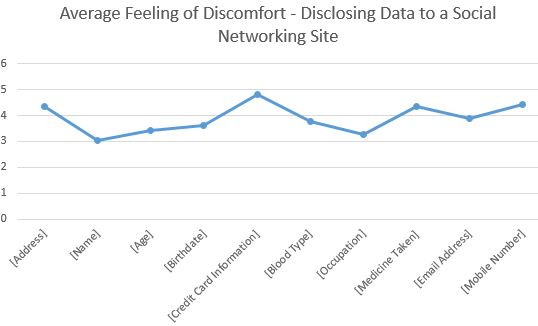
\includegraphics[width=0.5\textwidth]{Average_SocialNetworking}
\caption{Feeling of Discomfort in Disclosure - Social Networking application}
\end{center}
\end{figure}

\begin{figure}[h]
\begin{center}
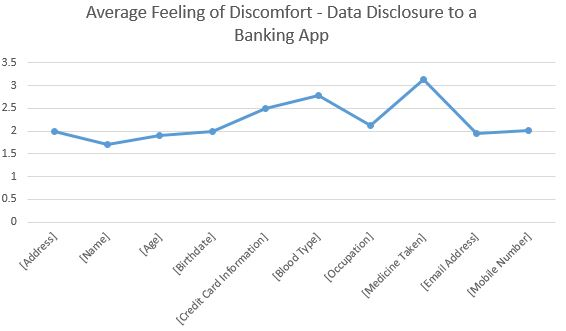
\includegraphics[width=0.5\textwidth]{Average_Banking}
\caption{Feeling of Discomfort in Disclosure - Banking application}
\end{center}
\end{figure}





\subsection{Qualitative analysis on factors that affect the feeling of discomfort in data disclosure}

Table 05 gives the summary of the codes we generated through the qualitative analysis. We developed a total of 11 codes.

\begin{center}
\begin{table*}[htbp]
\caption{Issues participants faced when embedding privacy into the designs}
\begin{center}
\begin{adjustbox}{width=1\textwidth}
\begin{tabular}{|p{0.20\linewidth}|p{0.64\linewidth}|p{0.16\linewidth}|}
\hline
Code &  Representative Quotes & Coverage (out of 151)\\
\hline
Benefit to me &how it benefits myself/ how useful it is for me. & 2.64\% (4)\\
\hline
How much I need the app &  based on my requirements from the application & 7.2\%(11)\\
\hline
News I see  & by considering cyber crimes and all that & 0.66\%(1) \\
\hline
Personal experience &  I was in couple of these situations which gave me an idea & 2\%(3) \\
\hline
Personal Safety & Some data are highly confidential and could end up in a reputational and/or financial loss/  don't like to see unwanted advertisements and messages & 12\% (19)\\ 
\hline
Relevance of data to the purpose &if I don't think such applications needs the data. For instance my blood group for a banking app
 & 26\% (40)\\ 
\hline
Visibility of Data - who can see it & audience with access to the data/ as in whether I could control what others see & 12\% (19)\\ 
\hline
Sensitivity of Data & As long as the requested information is not sensitive/  some sensitive information can't be disclosed irrespective of the application
 & 15\% (23)\\ 
\hline
Transparency - knowing how the data is used & Depends on what they are going to do with the information/ when privacy is not guaranteed & 6.6\% (10)\\ 
\hline
Trust with the application & every online application cannot be trusted/ random Facebook applications are not safe & 11\% (17)\\ 
\hline
Trust with the organization & If it is a reputed or a government institution there is less doubt and more trust on data security
 & 19\% (29)\\ 
\hline
\end{tabular}
\end{adjustbox}
\end{center}
\end{table*}
\end{center}

When it comes to data, participants mentioned only sensitivity, relevance and visibility of the data items that affect their disclosure decisions. Participants were most concerned about the relevance of data (26\%) followed by sensitivity of data (15\%) and visibility (12\%). Therefore, we could not identify any other factor related to data, that affects user disclosure decisions from the answers we received. 

However, we identified that users are concerned about the trust towards the organization that develop and publish applications (19\%). Participants said that they are comfortable sharing data as long as the application is developed and owned by a trusted organization. Some participants spoke about the trust with the application itself rather than the organization (11\%). Some participants also raised concerns about personal safety (12\%). Their concerns on personal safety was two fold. One was on financial and reputation loss on data being accessed by unknown parties. The other was their concern on being subjected to unwanted marketing via phone and email. They said that they consider this as a personal threat and hence they think twice before disclosing data to any application. A small number of participants were concerned about the previous personal experience and also about the benefit of sharing the data. 

\section{Discussion}

[to be decided]

\section {Limitations}

The study had several limitations. Firstly this was a remote survey. While remote surveys are beneficial in getting a large sample of participants in a relatively small period of time, direct engagement with users would disclose more in depth information when it comes to qualitative analysis. However, the main contribution of the paper was the derivation of the privacy measurement formula. Furthermore, for the qualitative component of data analysis we reached data saturation with the codes with 17 participants. The survey had 133 respondents which makes the results valid. Contextual studies involving real time applications that directly engage users in a natural setting could be used to observe how our findings stand in such setups.

Further, we did not intend to calculate the correlations in this survey. An interesting avenue to extend this survey would be to observe how data sensitivity, data relatedness and data visibility affects the disclosure decisions in particular. However, these parameters have been tested before in separate contexts, even though they do not have explicit reference to measuring properties in data against disclosure decisions. Therefore, we did not take it as a goal for this research.



\section{Conclusion and Future Work}




\iffalse

\begin{figure} 
\centering
\includegraphics [height=2 in,width=3 in]{Figure2.pdf}
\caption{Answer structure in a given security question \protect}
\vskip -6pt
\end{figure}
\fi

\iffalse 
Lying to a human being is a very bad thing to do, but, what if one lying to a computer to protect her privacy and keep her safe. 
\fi


\iffalse 
% no \IEEEPARstart
This demo file is intended to serve as a ``starter file''
for IEEE conference papers produced under \LaTeX\ using
IEEEtran.cls version 1.7 and later.
% You must have at least 2 lines in the paragraph with the drop letter
% (should never be an issue)
I wish you the best of success. 
\hfill mds
\hfill January 11, 2007

\subsection{Subsection Heading Here}
Subsection text here.


\subsubsection{Subsubsection Heading Here}
Subsubsection text here.
\fi




\iffalse 
\footnotesize
\bibliographystyle{abbrv}
\section{Conclusion}
The conclusion goes here. 




% conference papers do not normally have an appendix


% use section* for acknowledgement
\section*{Acknowledgment}


zzxzxz


\fi




\bibliographystyle{IEEEtran}
% argument is your BibTeX string definitions and bibliography database(s)
\bibliography{references}

\iffalse 
\begin{thebibliography}{1}

\bibitem{IEEEhowto:kopka}
H.~Kopka and P.~W. Daly, \emph{A Guide to \LaTeX}, 3rd~ed.\hskip 1em plus
0.5em minus 0.4em\relax Harlow, England: Addison-Wesley, 1999.

\end{thebibliography}




\section{Interview script}
Interview study 

\subsection*{ Demographics}

\begin{enumerate}
\item How old are you? ~\footnote{Most questions are open-ended questions}\\
\item How many people other than you live in your house?\\ 
\item What is each person's relationship to you?\\
\item What grade are you in school?\\
\end{enumerate}
\fi
\appendices

\section {Appendix A Survey Questionnaire}



% that's all folks
\end{document}



